% "Станет проще"

\documentclass[12pt]{article}

% report, book

%  Русский язык

\usepackage[T2A]{fontenc}
\usepackage[utf8]{inputenc}
\usepackage[english,russian]{babel}

\usepackage{geometry}
\geometry{a4paper}

\usepackage{amsmath,amsfonts,amssymb,amsthm,mathtools} 

\usepackage{graphicx}


\usepackage{wasysym}

\usepackage{geometry} 
\geometry{a4paper,top=2cm,bottom=3cm,left=2cm}



\begin{document} % начало документа

\newpage

\section{Система Лоренца}
Хаотическое поведение системы — такое поведение нелинейной системы, которое выглядит случайным, несмотря на то, что оно определяется конечным числом законов. 

Об объекте можно говорить, как о динамической системе, если можно указать такой набор величин, называемых динамическими переменными и характеризующих состояние системы, что их значения в любой последующий момент времени получаются из исходного набора по определенному правилу, называемым эволюцией системы.

Хоть и по определению динамической системы всегда можно однозначно предсказать конечное состояние по исходному, но в ней все равно может возникать хаос. В хаотическом режиме любая неточность в задании начального состояния нарастает во времени, так что предсказуемость становится недостижимой на достаточно больших интервалах времени. Такого рода режимы характеризуются нерегулярным, хаотическим изменением динамических переменных во времени.

Точки, представляющие состояние динамической системы в последовательные моменты времени в течение всего времени эволюции, образуют кривую в фазовом пространстве. Эта кривая называется фазовой траекторией. 

Модель Лоренца является реальным физическим примером динамических систем с хаотическим поведением, в отличие от различных искусственно сконструированных отображений.

Система уравнений имеет вид
$$\begin{cases}	
	\dot{x} = \sigma (y-x) \\
	\dot{y} = x(\rho-z)-y \\
	\dot{z} = xy-bz
\end{cases}$$

Эта модель была впервые описана в 1963 году Эдвардом Лоренцом в статье "Детерминированное непериодическое течение". Лоренц получил эту модель как линейную аппроксимацию гидродинамической системы уравнений для задачи о конвекции морской воды в плоском слое; значения параметров и начальные условия были выбраны таким образом: $\sigma = 10$, $\rho = 28$, $b = \frac{8}{3}$; $x(0) = 1$, $y(0) = 0$, $z(0) = 0$.

Для любого решения системы Лоренца существует такой момент времени, когда соответствующая фазовая траектория навсегда погружается в эллипс фиксированного размера (про это в параграфе 3). Поэтому существует предельное множество, к которому притягиваются все траектории динамической системы при $t \rightarrow \infty$. Поэтому можно говорить, что аттрактор Лоренца ― \textbf{компактное инвариантное множество} (сфера -- компакт) L в трехмерном фазовом пространстве гладкого потока. Таким образом, аттрактор определяет поведение решений системы Лоренца на больших отрезках времени.

\section{Конвекция в замкнутой петле}

Трубка, замкнутая в кольцо, наполнена почти несжимаемой жидкостью. Она подогревается снизу и охлаждается сверху, и при достаточно сильном нагреве возможно возникновение конвекционного течения.

\begin{figure}[h]
	\centering
 	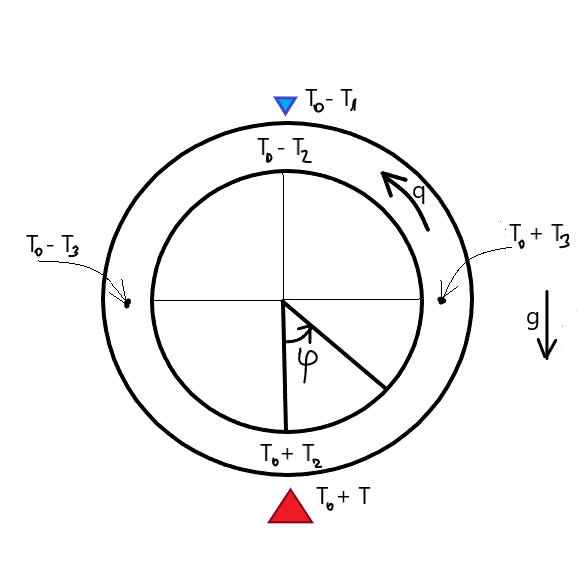
\includegraphics[scale=0.365]{Lorenz.png}
 	\caption{Кольцо с подогревом.}
\end{figure}

Пусть $a$ -- радиус петли, внутренний радиус много меньше $a$.

Заметим, что раз жидкость почти несжимаемая, то ее скорость во всех точках трубки постоянна, она не зависит от $\phi$. Обозначим скорость за $q = q(t)$.

Температура жидкости в трубке будет зависить от угла $\phi$, который отсчитывается от направленного вниз радиуса до точки против часовой стрелки. $T = T(\phi) -$ периодическая функция (период равен $2\pi$) $\Rightarrow$ ее можно разложить в ряд Фурье.

При разложении основную амплитуду задают первые слагаемые, поэтому рассмотрим только первую гармонику. Уравнение будет иметь вид 
\begin{equation}\label{eq1}
T - T_0 = T_2\cos\phi + T_1\sin\phi
\end{equation}
Исследуем коэффициенты при $\sin\phi$ и $\cos\phi$.

Рассмотрим $\phi = 0$ и $\phi = 2 \pi$, тогда $\cos\phi = 1, \sin\phi = 0$. Значит, $2T_2$ показывает разницу температур между нижней точкой (точка нагрева) и верхней точкой (точка охлаждения). Аналогично исследуем при $\phi = \frac{\pi}{2}$ и $\phi = \frac{3 \pi}{2}$. Получается, что $2T_3$ отвечает за разницу между боковыми точками петли. $T_2$ и $T_3$ зависят от времени.

Уравнение Навье-Стокса в общем виде:

\begin{equation*}
\frac{\partial \overrightarrow{u}}{\partial t} + \overrightarrow{u} \cdot \overrightarrow{\nabla} \overrightarrow{u} = -\frac{1}{\rho} \overrightarrow{\nabla} p - \overrightarrow{g} \alpha \Delta T + v \nabla^2 \overrightarrow{u}
\end{equation*}

В наших обозначениях:
\begin{itemize}
\item $\overrightarrow{u} \rightarrow q$
\item так как $q=q(t)$, то можно заменить $\frac{\partial q}{\partial t}$ на $\frac{dq}{dt}$
\item жидкость несжимаемая, следовательно $\overrightarrow{u} \cdot \overrightarrow{\nabla} \overrightarrow{u} \rightarrow 0$
\item при переходе в полярные координаты $\overrightarrow{\nabla} p \rightarrow \frac{1}{a} \frac{\partial p}{\partial \phi}$
\item коэффициент кинематической вязкости $\Gamma$ зависит от скорости, поэтому $v \nabla^2 \overrightarrow{u} \rightarrow -\Gamma q$
\end{itemize}


В каждой точке кольца действует сила Архимеда, она состоит из нормальной и тангенциальной составляющей. Нормальная составляющая компенсируется стенками, поэтому рассмотрим тангенциальную (понятно, что численно $F_{\theta} = F\sin\phi$). Рассмотрим на глубине $h$ слой толщиной $dh$. Объем, а значит и плотность, зависят от температуры, то есть зависят от глубины 

$-\overrightarrow{g} \alpha \Delta T = g \alpha (T-T_0) \sin\phi$

В итоге, уравнение Навье-Стокса для нашей системы примет вид:

\begin{equation}\label{eq2}
\frac{\partial q}{\partial t} = -\frac{1}{\rho a}\frac{\partial p}{\partial \phi} + g \alpha (T-T_0) \sin\phi -\Gamma q
\end{equation}

Подставим уравнение (\ref{eq1}) в (2):

\begin{equation*}
\frac{\partial q}{\partial t} = -\frac{1}{\rho a}\frac{\partial p}{\partial \phi} + g \alpha (T_2\cos\phi + T_1\sin\phi) \sin\phi -\Gamma q
\end{equation*}

Избавимся от части с давлением, проинтегрировав один раз от 0 до $2\pi$. Тогда 

\begin{equation*}
-\frac{1}{\rho a} \int_{0}^{2\pi} \frac{\partial p}{\partial \phi}\, d\phi = 0
\end{equation*}

\begin{equation*}
g \alpha T_2 \int_{0}^{2\pi} \cos\phi \sin\phi\, d\phi = \frac{1}{2} \sin^2 \phi \Big|_0^{2\pi} = 0
\end{equation*}

\begin{equation*}
g \alpha T_3 \int_{0}^{2\pi} \sin^2 \phi\, d\phi = g \alpha T_3 \pi
\end{equation*}

\begin{equation*}
\int_{0}^{2\pi} \frac{\partial q}{\partial t}\, d\phi = 2\pi
\end{equation*}

\begin{equation*}
\int_{0}^{2\pi} -\Gamma q\, d\phi = -2\pi\Gamma q
\end{equation*}

Тогда, поделив обе части уравнения на $2\pi$, получим:

\begin{equation}\label{eq23}
\frac{dq}{dt} = -\Gamma q + \frac{g \alpha T_3}{2}
\end{equation}

Таким образом, можно заметить, что скорость изменяется из-за разницы температур в боковых точках, то есть зависит от $2T_3$.

Теперь рассмотрим уравнение распространения теплоты в жидкости:

\begin{equation*}
\frac{\partial T}{\partial t} + \overrightarrow{u} \overrightarrow{\nabla} T = \kappa \nabla^2 T 
\end{equation*}
где $\kappa$ -- коэффициент температуропроводности.

В условиях задачи:

\begin{equation}\label{eq3}
\frac{\partial T}{\partial t} + \frac{q}{a} \frac{\partial T}{\partial \phi} = K(T_{external}-T_{internal}) = K(T_E-T)
\end{equation}

Внешняя температура зависит от высоты: 
\begin{equation}\label{eq4}
T_E = T_0+T_1\cos\phi
\end{equation}
Внутренняя же температура зависит от $T_2$ и $T_3$ (уравнение (\ref{eq1})). Вычтем из (\ref{eq1}) (4) и подставим в (3):

\begin{equation*}
\frac{dT_2}{dt}\cos\phi + \frac{dT_3}{dt}\sin\phi - \frac{q}{a}T_2\sin\phi + \frac{q}{a}T_3\cos\phi = K(T_1-T_2)\cos\phi-KT_3\sin\phi
\end{equation*}

Коэффициенты при $\sin\phi$ и $\cos\phi$ должны совпадать в обеих частях, следовательно 

\begin{equation*}
\frac{dT_3}{dt} - \frac{qT_2}{a} = -KT_3
\end{equation*}

\begin{equation*}
\frac{dT_2}{dt} + \frac{qT_3}{a} = K(T_1-T_2) = KT_4
\end{equation*}
где $T_4$ показывает разницу внешней и внутренней температуры внизу и вверху трубки.

\begin{equation}\label{eq5}
\frac{qT_2}{a} = \frac{qT_1}{a} - \frac{qT_4}{a} \Longrightarrow \frac{dT_3}{dt} = -KT_3 + \frac{qT_1}{a} - \frac{qT_4}{a}
\end{equation}

$T_1$ определяется конфигурацией системы и не зависит от времени, следовательно, $\frac{dT_2}{dt} = -\frac{dT_4}{dt} \Longrightarrow$

\begin{equation}\label{eq6}
\frac{dT_4}{dt} = -KT_4 + \frac{qT_3}{a}
\end{equation}

Уравнения (3), (6) и (7) образуют систему дифференциальных уравнений, которую можно привести к виду системы Лоренца. Для этого сделаем следующие замены:
\begin{equation*}
q = aKx, \quad T_3 = \frac{2a \Gamma Ky}{g \alpha}, \quad T_4 = \frac{2a \Gamma Kz}{g \alpha}, \quad t \rightarrow Kt
\end{equation*}

Тогда

\begin{equation*}
aK^2\dot{x} = -\Gamma aKx + a\Gamma Ky \Longrightarrow \dot{x} = \frac{\Gamma}{K} (y - x)
\end{equation*}

\begin{equation*}
\frac{2a\Gamma K^2}{g\alpha} \dot{y} = -\frac{2a\Gamma K^2}{g\alpha}y + \frac{aKxT_1}{a} - \frac{aKx \cdot 2a \Gamma Kz}{ag\alpha} \Longrightarrow \dot{y} = -y + \frac{g\alpha T_1}{2a\Gamma K}x - xz
\end{equation*}

\begin{equation*}
\frac{2a\Gamma K^2}{g\alpha} \dot{z} = -\frac{K \cdot 2a\Gamma K}{g\alpha} + \frac{aKx \cdot 2a\Gamma Ky}{a} \Longrightarrow \dot{z} = -z+xy
\end{equation*}


Таким образом, была получена система дифференциальных уравнений Лоренца.
$$\begin{cases}	
	\dot{x} = \sigma (y-x) \\
	\dot{y} = x(\rho-z)-y \\
	\dot{z} = xy-bz
\end{cases}$$
где 
\[ \rho = \frac{g\alpha T_1}{2a\Gamma K} - \text{число Рэлея}\]
\[P = \frac{\Gamma}{K} - \text{число Прандтля}\] 
\[b = 1 \text{, так как рассматриваем кольцо}\]

Число Релея определяет поведение жидкости под воздействием градиента температуры. Число Прандтля -- один из критериев подобия тепловых процессов в жидкостях, который учитывает флияние физических свойств теплоносителя на теплоотдачу.

В условиях данной задачи $x$ показывает скорость течения, $y$ -- отклонение температуры от средней в точке $\phi = \frac{\pi}{2}$, $z$ -- то же, но в нижней точке.

\section{Аналитическое исследование}

\begin{enumerate}
\item Заменим одновременно знак у $x$ и $y$:
\begin{equation*}
\dot{(-x)} = \sigma(-y-(-x)) \Leftrightarrow -\dot{x}=-\sigma(y-x) \leftrightarrow \dot{x}=\sigma(y-x)
\end{equation*}
\begin{equation*}
\dot{(-y)} = -x(\rho-z)-(-y) \leftrightarrow -\dot{y}=-(x(\rho-z)-y) \Leftrightarrow \dot{y}=x(\rho-z)-y
\end{equation*}
\begin{equation*}
\dot{z} = -bz+(-x)(-y) \Leftrightarrow \dot{z}=-bz+xy
\end{equation*}
Заметно, что система уравнений \textit{симметрична}. Это значит, что любое образование в фазовом пространстве обладает той же симметрией, то есть превращается само в себя при замене переменных.

\item Пусть $w=\rho-z$, тогда система уравнений принимает вид:
$$\begin{cases}	
	\dot{x} = \sigma (y-x) \\
	\dot{y} = xw-y \\
	\dot{w} = -bw+b\rho-xy
\end{cases}$$
Домножим $\dot{x}$ на $\frac{x}{\sigma}$, $\dot{y}$ на $y$, $\dot{w}$ на $w$ и сложим:
\begin{equation*}
\frac{x}{\sigma}\frac{dx}{dt}+y\frac{dy}{dt}+w\frac{dw}{dt}=xy-x^2-y^2+xyw-bw^2-xyw+b\rho w
\end{equation*}
\begin{equation*}
\frac{d}{dt}\left(\frac{x^2/\sigma+y^2+w^2}{2}\right)=-\left(x-\frac{1}{2}y\right)^2-\frac{3}{4}y^2-b\left(w-\frac{1}{2}\rho\right)^2+\frac{1}{4}b\rho^2
\end{equation*}
В трехмерном пространстве $(x, y, w)$ область, заданная неравенством $RHS \geqslant 0$, ограничена поверхностью параллелепипеда, смещенного относительно начала координат. А значит вне этой области $RHS < 0$.
Определим множество эллипсоидов в этом же пространстве, заданных уравнением $x^2/\sigma+y^2+w^2=const$, и возьмем такую константу, чтобы полученный эллипсоид полностью содержал в себе область, описанную выше. Тогда на поверхности эллипсоида всюду $\frac{d}{dt}(x^2/\sigma+y^2+w^2) < 0$, то есть величина $x^2/\sigma+y^2+w^2$ убывает. Значит, все траектории, пересекающие поверхность эллипса, ведут только внутрь ограниченной им области. То есть в какой-то момент времени любая фазовая траектория погружается в эллипс с фиксированными параметрами.

\item Система имеет \textit{неподвижные точки} (состояния равновесия). Это такие состояния, которые не меняются во времени, то есть $\dot{x}, \dot{y}, \dot{z}$ обращаются в нуль.
$$\begin{cases}
0=\sigma(x-y) \\
0=\rho x-y-xz \\
0=-bz+xy
\end{cases}
\Rightarrow
\begin{cases}
x=y \\
x(\rho-1-z)=0 \\
x=\pm\sqrt{bz}
\end{cases}$$
1 случай: $x=0$, тогда $z=0$. 2 случай: $z=\rho-1$, тогда $x=\pm\sqrt{\rho-1}$, понятно, что 2 случай возможен только при $\rho \geqslant 1$. 
\\ Значит, при $r < 1$ возможно только одно состояние равновесия:
\begin{equation*}
x=0, \quad y=0, \quad z=0
\end{equation*}
При $r \geqslant 1$ будет три состояния равновесия (первое см. выше):
\begin{equation*}
x=\sqrt{\rho-1}, \quad y=\sqrt{\rho-1}, \quad z=r-1
\end{equation*}
\begin{equation*}
x=-\sqrt{\rho-1}, \quad y=-\sqrt{\rho-1}, \quad z=r-1
\end{equation*}
Физический смыл точки $(0, 0, 0)$ -- отсутствие конвекционных потоков. Другие две точки соответствуют наличию конвекционного потока против часовой стрелки для второй точки и против -- для третьей. Стоит отметить, что вторая и третья точки являются симметричными, что является примером к первой рассмотренной особенности системы Лоренца.

\item Неподвижная точка будет \textit{устойчивой}, если для любого $\epsilon > 0$ существует такое $\delta > 0$, что для любых начальных данных из $\delta$-окрестности точки вся траектория системы содержится в $\epsilon$-окрестности точки. Неподвижная точка \textit{неустойчивая}, если это условие не выполняется. Линейно проанализируем найденные неподвижные точки на устойчивость. Для этого произведем замены: $x=x_0+\tilde{x}, \quad y=y_0+\tilde{y}, \quad z=z_0+\tilde{z}$, где тильды зависят от времени и считаются малыми. Тогда произведение пары тильд будет малым, и им можно пренебречь. Тогда система Лоренца будет иметь вид:
$$\begin{cases}
\dot{\tilde{x}} = \sigma(\tilde{y}-\tilde{x}) \\
\dot{\tilde{y}} = \rho\tilde{x}-\tilde{y}-x_0\tilde{z}-z_0\tilde{x} \\
\dot{\tilde{z}} = -b\tilde{z}+x_0\tilde{y}+y_0\tilde{x}
\end{cases}$$ 
Зависимость возмущения от времени экспоненциальная (особенность анализа), то есть  $ \tilde{x}, \tilde{y}, \tilde{z} \sim exp(\lambda)$. Тогда уравнение принимает вид:
\begin{equation*}
\lambda
\begin{pmatrix}
\tilde{x} \\
\tilde{y} \\
\tilde{z}
\end{pmatrix}
=
\begin{pmatrix}
-\sigma & \sigma & 0\\
\rho-z_0 & -1 & -x_0 \\
y_0 & x_0 & -b
\end{pmatrix}
\end{equation*}
Нетривиальное решение существует, если определитель будет равен нулю:
\begin{equation*}
\begin{vmatrix}
\lambda+\sigma & -\sigma & 0\\
-\rho+z_0 & \lambda+1 & x_0 \\
-y_0 & -x_0 & \lambda+b
\end{vmatrix}
=0
\end{equation*}
то есть
\begin{equation*}
(\lambda+\sigma)((\lambda+1)(\lambda+b)+x_0^2)+\sigma((\lambda+b)(z_0-\rho)+x_0y_0)=0
\end{equation*}
Точка будет устойчивой, если все три собственных числа отрицательны (для комплексных -- вещественная часть отрицательна), и неустойчивой в иных случаях.
\\ Подставим первую неподвижную точку $(0, 0, 0)$:
\begin{equation*}
(\lambda+\sigma)(\lambda+1)(\lambda+b)-\sigma\rho(\lambda+b)=0
\end{equation*}
\begin{equation*}
(\lambda+\sigma)(\lambda^2+(\sigma+1)\lambda+\sigma(1-\rho))=0
\end{equation*}
\begin{equation*}
\Rightarrow \quad \lambda_1=-b, \quad \lambda_{2,3}=\frac{-(\sigma+1)\pm\sqrt{(\sigma+1)^2+4\sigma(1-\rho)}}{2}
\end{equation*}
$\lambda_1$ всегда отрицательно, $\lambda_{2,3}$ отрицательны при $\rho<1$, так как тогда выражение под корнем будет больше $(\sigma+1)^2$. При $\rho>1$ одно из решений становится положительным. То есть точка $(0, 0, 0)$ устойчива при $\rho<1$ и неустойчива при $\rho>1$.
\\ Оставшиеся две точки существуют только при $r>1$. Подставим их в уравнение на $\lambda$:
\begin{equation*}
(\lambda+\sigma)(\lambda^2+\lambda b+\lambda+b+b\rho-b)+\sigma((\lambda+b)(\rho-1-\rho)+b\rho-b)=0
\end{equation*}
\begin{equation*}
(\lambda+\sigma)(\lambda^2+\lambda b+\lambda+b\rho)+\sigma(-\lambda+b\rho-2b)=0
\end{equation*}
\begin{equation*}
\lambda^3+\lambda^2(b+\rho+1)+\lambda b(\rho+\sigma)+2b\sigma(\rho-1)=0
\end{equation*}
Исследования показали, что при $\rho=1+\epsilon$ все три собственных числа отрицательны, следовательно, неподвижные точки являются устойчивыми. При увеличении $\rho$ с некоторого момента одно собственное число будет действительным и отрицательным, а два других -- комплексно-сопряженные с отрицательной $Re$, точки все еще остаются устойчивыми (но другого вида). При дальнейшем увеличении $\rho$ действительная часть меняет знак, и это момент потери устойчивости точек.

\end{enumerate}

\section{Бифуркация}

Бифуркация -- приобретение нового качества эволюции
динамической системы при малом изменении ее параметров.
Бифуркация соответствует перестройке характера движения
или структуры системы.

Рассмотрим изменение динамики системы при изменении параметра $\rho$ (для конвекции в петле -- изменение нагрева). 

При $\rho<1$ есть одна устойчивая неподвижная точка $(0, 0, 0)$ -- это единственный аттрактор системы (по определению аттрактора -- подмножество фазового пространства, все траектории из некоторой окрестности которого стремятся к нему при $t \rightarrow \infty$). 

При $\rho>1$ состояние равновесия в $(0, 0, 0)$ становится неустойчивым. Введя малое возмущение, изображающая точка будет уходить от состояния равновесия вдоль некоторой специальной траектории (кривой линии) -- неустойчивого многообразия, или сепаратрисы. Оно одномерное, так как только одно собственное число становится неотрицательным, следовательно, только одно число ответственно за неустойчивость. При этом будет кривая поверхность (устойчивое многообразие), при старте с которой траектории будут идти в состояние $(0, 0, 0)$. Это будет поверхность, так как два собственных числа отрицательны.

После перехода $\rho$ через значение 1, $(0, 0, 0)$ перестает быть устойчивой, следовательно, уже не аттрактор. Но аттракторами становятся две возникшие неподвижные точки (соответствуют состояниям с равномерным вращением жидкости), которые остаются устойчивыми до каких-то значений $\rho$. Два аттрактора означают наличие бистабильности -- система может прийти в конце в один из двух возможных устойчивых режимов (зависит от начальных условий). 

При этом фазовые траектории будут приближаться к неподвижной точке по спирали, и чем больше $\rho$, тем больше начальный размах спирали. Исследования показали, что при $\rho=13.927$ неустойчивое многообразие совершает один оборот и приходит в точку $(0, 0, 0)$ вдоль оси $Oz$ -- петля сепаратрисы. В этот момент происходит перестройка потока фазовых траекторий (\textit{нелокальная бифуркация}), не сводящаяся к локальным изменениям в окрестности какой-то одной точки фазового пространства. В условиях задачи про петлю это соответствует явлению, что при установлении режима конвекции, начиная от ситуации вращения с малой скоростью, направление движения жидкости меняется на противоположное.

Следующая существенная нелокальная бифуркация происходит при $\rho \approx 24.06$. С этого момента возникает притягивающее множество сложной структуры, которое и является странным аттрактором Лоренца, отвечающим хаотическому режиму колебаний. При этом, состояния, рассмотренные до этого, все еще остаются устойчивыми до $\rho=24.74$. Таким образом, в этот промежуток значений $\rho$ в системе сосуществуют три аттрактора. После $\rho=24.74$ точки теряют свою устойчивость, и в системе остается единственное притягивающее -- аттрактор Лоренца.

\section{Другие области применения}

Модель Лоренца применима в других физических процессах:
\begin{itemize}
	\item Конвекция в плоском слое
	\item Вращение водяного колеса (колесо, на ободе которого укреплены корзины с отверстиями в дне; сверху на колесо симметрично относительно оси вращения льётся сплошной поток воды)
	\item Одномодовый лазер
	\item Диссипативный осциллятор с инерционным возбуждением
\end{itemize}

При этом в других моделях переменные и параметры будут иметь другой смысл. Так для конвекции в плоском слое $x$ отвечает за скорость вращения водяных валов, $y$ и $z$ -- за распределение температуры по горизонтали и вертикали, $\rho$ -- нормированное число Рэлея, $\sigma$ -- число Прандтля (отношение коэффициента кинематической вязкости к коэффициенту температуропроводности), $b$ содержит информацию о геометрии конвективной ячейки. 

Вращение водяного колеса похоже по поведению на конвецкцию в замкнутой петле с точностью до переворота "вверх ногами"\,, поэтому описывается аналогичными уравнениями с заменой температуры на плотность распределения массы воды в корзинах по ободу.

Для одномодового лазера $x$ -- амплитуда волн в резонаторе лазера, $y$ -- поляризация, $z$ -- инверсия населённостей энергетических уровней, $b$ и $\sigma$ -- отношения коэффициентов релаксации инверсии и поля к коэффициенту релаксации поляризации, $\rho$ -- интенсивность накачки.


\end{document} % конец документа